% !Mode::"Tex:UTF-8"

\documentclass[a4paper]{article}
\usepackage{ctex}
\author{刘军(NUFE,210042)}
\date{}
\title{Incremental learning for Fast Discrimination of complex compound base on SVM and convex hull vectors }
\usepackage{amssymb}    %使用宏包{美国数学协会符号}
\usepackage{amsmath}
\usepackage{multirow}
% 页面设置
\usepackage[top=2.54cm,bottom=2.54cm,left=3.18cm,right=3.18cm]{geometry}
% 页眉页脚设置
\usepackage{fancyhdr}
\pagestyle{fancy}
\lhead{Incremental learning for Fast Discrimination of complex compound base on SVM and convex hull vectors}
%\chead{\thesection}
\cfoot{\thepage}
% 插图包,两个图并排
\usepackage{graphicx}
\usepackage{subfigure}

\begin{document}
\maketitle


Abstract:using new samples to improve the accurate of classification for complex compound such as apple essence is a key aspect for rapidly and accurate determination in online detection.In this paper,a novel methodology is proposed,which involves two crucial aspects in the context of the use of online data in classification for complex compound:i)the method of the complex compound resolution for online data by incremental learning algorithm based on Hull vector;and ii)the selection of the most appropriate spectroscopy,taking into account both 识别风险 和 代价、分辨率等.Both Raman and ion mobility spectrometry (IMS) had the advantages of easy operation and  quick  analysis.It was shown that the identification accuracy rate of the Raman spectroscopy for nine kinds of apple essences was 98.35\%,which is higher then that of the IMS.The results from this study demonstrated that the Raman spectroscopy combined with incremental learning algorithm can be used as a reliable,stable and fast new method to discriminate among complex compound.

Key words:Apple Essences;Incremental Learning;Convex hull;SVM;discrimination
%=============第一部分 简介===================
\section{I. Introduction}

    \subsection{discrimination of complex compound}
    % 苹果香精检测的背景、
Natural apple essence is restricted by geography, climate, species, artificial conditions and other factors, facing unstable product quality, serious loss of raw materials, short supply and low concentration.Synthetic apple essence is widely used because of its controllable formula, stable product quality and relatively low price.The quality of essence is controlled mainly by refractive index, relative density, acidity degree value, total volatile component, physical-chemical indexes and sensory evaluation.The former can only reflect some characteristics of essences, and it has many disadvantages, such as excessive test items, complicated operation, long detection time, low efficiency and so on.The latter uses nose feeling as an identification tool, which can not accurately reflect the quality fluctuation of essence, is easily affected by the sensory evaluation staff level, physical state and environmental factors.So whether to provide a more reliable and stable detection of new methods, has attracted the attention of researchers.At present, the quality evaluation of apple essence focused on  the major aroma components,common detection means as an electronic nose, gas chromatography, gas chromatography - mass spectrometry and the like.These methods play an important role in the quality control of apple essence, but there are also some defects, such as a single indicator, not adapt to the characteristics of essence diversification, high cost, long analysis time,can not effectively achieve rapid essence analysis and process control.

Raman spectroscopy is a rapid detection method developed in recent years, with fast, efficient, non-polluting, without pre-treatment, lossless analysis, etc., many areas have been widely used.

    \subsection{Incremental SVM Learning Base on Hull Vector}
    \subsubsection{Standard SVM overview}
Support Vector Machines(SVM) $^{\cite{Vapnik}}$ have been successfully used for machine learning with large and high dimensional data sets. This is due to the fact that the generalization property of an SVM does not depend on the training data but only a subset thereof, the so called support vectors.

The normal SVM classifiers learned from the data $\{ (x_i,y_i)\in\ \mathbb{IR}^m \times \{ -1, 1 \} ,\forall i \in \{ 1,\cdots,N \} \}$ by minimizing
% 公式1
% \符号可以用来半个空格
\begin{equation}
\min \limits_{w,b,\xi} \ \ \frac{1}{2}||w||^2+C\sum^{N} \limits_{i=1}\xi_i \tag{1}
\end{equation}


$$
s.t. \ \ y_i(w^T x_i + b)\geq 1-\xi_i,
$$
$$
\ \ \ \ \xi_i \geq  0 \ ,\forall \ i \in \{1,\cdots,m\}
$$

for learning nonlinear SVM, With Lagrange multiplier the quadratic program is typically expressed in its dual form:
% 公式2
\begin{equation}
\max_a  \sum_{i=1}\limits^{m} \alpha_i - \frac{1}{2} \sum \limits^{m} \limits_{i=1} \sum \limits^{m} \limits_{j=1} \alpha_i \alpha_j y_i y_j x_i^T x_j \tag{2}
\end{equation}

$$
s.t. \ \ \sum \limits_{i=1} \limits^{m} \alpha_i y_i = 0 ,
$$
$$
     \qquad \qquad \qquad \qquad \qquad 0\leq \alpha_i \leq C, ,\forall \ i \in \{1,\cdots,m\}
$$

SVM uses kernel function  $K(x,y)= \langle\phi(x) , \phi(y)\rangle =\phi(x) \cdot \phi(y) = \phi(x)^T  \phi(y)$  to instead of point multiply in high dimensional feature space, perfectly solving the dimension problem.The resulting form of SVM is :
\begin{equation}
f(x) = \sum \limits_{i=1} \limits^{m} \alpha_i y_i k(x_i,x) + b \tag{3}
\end{equation}

By solving the dual optimization problem ,the required classification discriminant function is obtained,such as ;
\begin{equation}
f(x) = sgn( w \cdot x + b ) = sgn \left|\sum \limits_{i=1} \limits^{m} y_i \alpha_i \cdot k(x_s,x_i)+b^*  \right|   \tag{4}
\end{equation}

In the above formula, $x_i$ is a support vector, $x$ is a sample that need to classified,the dimension of W is is equal to feature space's.

    \subsubsection{Incremental SVM Learning Base on Hull Vector}

However,the normal SVM algorithm does not support incremental learning.The classification process usually face the new evolving data,the initial training sample set can not reflect all the sample information.When new training samples are accumulated to a certain scale, in order to obtain the new sample information,we would like to integrate these examples and train a new classification model.
A standard SVM has time complexity of order $O(M^3)$(M is the number of training samples)Obviously,the drawback does benefit large-scale online applications.

To attack this problem,lots of works have been done.One way is to reduce training samples with a certain sample selection strategy.The quality of training data set is vital to the performance of the classifier being constructed.Syed et al.$ ^{\cite{Stefan}}$ worked out an incremental algorithm based on SVM, which retains only the support vector set as a historical training sample.XIAO Rong et al. $ ^{\cite{XIAORong}}$ studies the distribution law of new data and existing data,focus on  the characteristics of the support vectors,through the introduction of weights to select samples.Shin and Cho $^{\cite{yunjungShin}}$presented a pattern selection algorithm to choose the samples near separation margins for constructing new training sets.Lee and Huang et al. \cite{YJLee} randomly selected a portion of data set as to generate a thin rectangular kernel matrix, and they used this much smaller rectangular kernel matrix to replace the full kernel matrix in the nonlinear SVM formulation.

%=============第二部分 实验与材料===================
\section{II.Experiments and Materials}
A total of 27 experimental samples, corresponding to three apple essence brands,were obtained from three famous flavors and fragrances companies in China by three batches.All samples were produced in 2016,and had equivalent proofs.The apple essence included in study are listed in Table1.
%\left(
%  \begin{array}{Detailed information of the investigated apple essences}
%    flavor companies & no. & solvent \\
%    A & S & ethanol \\
%  \end{array}
%\right)

\begin{table}{h} %开始一个表格environment,表格的位置是h,here
  \centering
  \caption{Detailed information of the investigated apple essences}\label{a}
  \begin{tabular}{c|c|l}

     \hline
     % after \\: \hline or \cline{col1-col2} \cline{col3-col4} ...
     flavor companies       & no.       & solvent \\
     \hline
     \multirow{3}{*}{A}       & S         & ethanol \\
     \cline{2-3}
                              & Q         & ethanol \\
     \cline{2-3}
                              & I         & 1,2 propanediol \\
     \hline
     \multirow{3}{*}{B}       & a         & 1,2 propanediol \\
     \cline{2-3}
                              & b         & ethanol,1,2 propanediol \\
     \cline{2-3}
                              & c         & 1,2 propanediol,water \\
     \hline
     \multirow{3}{*}{C}       & d         & 1,2 propanediol \\
     \cline{2-3}
                              & e         & ethanol \\
     \cline{2-3}
                              & f         & 1,2 propanediol \\
     \hline
   \end{tabular}

\end{table}



\subsection{Materials and Reagent}

\subsection{Instrument and Equipment}



\begin{figure}[h]
  \centering
  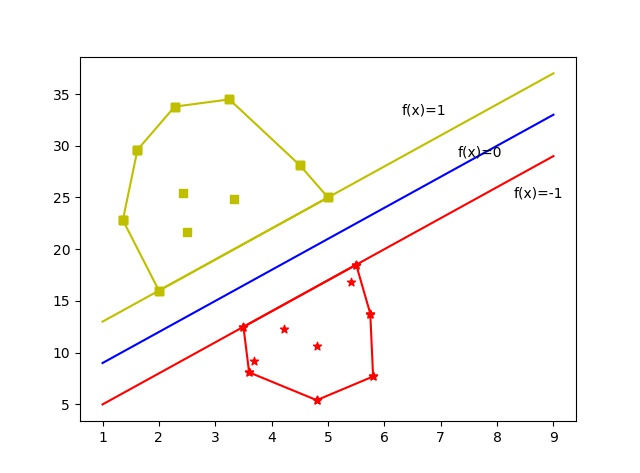
\includegraphics[width=9cm,height=6cm]{HullVector_SupportVector}
  \caption{Relationship between hull vectors and support vectors}
\end{figure}


% 方法
\subsection{Methods}
% 样品制备
\subsubsection{Sample Preparation}
% 谱图采集
\subsubsection{Spectrum acquisition}

% 数据处理
\subsection{Data processing}


%=============第三部分 数据分析===================
\section{III. Data Analysis}
% 拉曼数据分析
\subsection{Raman spectrum Data analysis}
% IMS数据分析
\subsection{IMS Data analysis}

%=============第四部分 结果与分析===================
\section{IV. Result and Discussion}


%=============第五部分 结论===================
\section{V.	Conclusion}


\renewcommand\refname{References}
\begin{thebibliography}{99}
    \bibitem{Vapnik}V.N. Vapnik, The Nature of Statistical Learning Theory, Springer, New York,1995, 8 (6) :988 - 999
    \bibitem{Stefan}Stefan Ruping,Incremental Learning with Support Vector Machines,Technical Reports,2001,228(4):641-642
    \bibitem{XIAORong}XIAO Rong, WANG Ji-cheng, SUN Zheng-xing. Anapproach to incremental SVM learning algorithm.Journal of Nanjing University, 2002, 38(2): 152 157.
    \bibitem{Zhu X}Zhu X, Lafferty J, Ghahramani Z. Combining active learning and semi-supervised learning using Gaussian fields  and  harmonic  functions[C].  In:  Proc  of  ICML  2003  Workshop  on  the  Continuum  from  Labeled  to Unlabeled Data. Menlo Park, CA:AAAI Press,2003:58-65.
    \bibitem{yunjungShin}Hyunjung Shin, Sungzoon Cho, Invariance of neighborhood relation underinput space to feature space mapping, Pattern Recognition Letters, 26 (2005)707–718.
    \bibitem{YJLee}Y.J. Lee, S.Y. Huang, Reduced support vector machines: a statistical theory,IEEE Transactions on Neural Networks 18 (No.1) (2007) 1–13.
\end{thebibliography}


\end{document}

